\documentclass[12pt]{beamer}

\usepackage{algorithm}
\usepackage[noend]{algorithmic}
\usepackage[english]{babel}
\usepackage[utf8]{inputenc}
\usepackage{tabularx}
\usepackage{textcomp}
\usepackage{tikz}
\usepackage{xspace}

\usetheme{Copenhagen}
\setbeamertemplate{navigation symbols}{}
\setbeamertemplate{bibliography entry title}{}
\setbeamertemplate{bibliography entry location}{}
\setbeamertemplate{bibliography entry note}{}

\bibliographystyle{amsalpha}

\renewcommand{\algorithmicrequire}{\textbf{Input:}}
\renewcommand{\algorithmicensure}{\textbf{Output:}}
\renewcommand{\algorithmiccomment}[1]{/\(\!\)/ #1}

\newcommand{\textapprox}{\raisebox{0.5ex}{\texttildelow}}
\newcommand{\pp}{\nolinebreak\hspace{-.05em}\raisebox{.4ex}{\tiny\bf +}\nolinebreak\raisebox{.4ex}{\tiny\bf +}\xspace}

\title[Traversing the \(k\)-mer Landscape of NGS Read Datasets]{
    Traversing the \(k\)-mer Landscape of NGS Read Datasets for Quality Score Sparsification
}
\author[Jacopo Notarstefano]{
    Jacopo Notarstefano\\
    \texttt{jacopo.notarstefano [at] gmail.com}
}
\date{May 19, 2014}

\begin{document}
    \begin{frame}[plain]
        \titlepage
    \end{frame}

    \begin{frame}{Next-generation sequencing (NGS)} 
        NGS is the name given to several different sequencing technologies that
        were developed in the past decade.

        \vspace{0.5cm}

        These methods have in common a much higher throughput and a much lower
        cost compared to Sanger sequencing, which was used to sequence the
        Human Genome \cite{LLL12}.

        \vspace{0.125cm}

        \begin{table}
            \centering
            \begin{tabularx}{\linewidth}{lccc}
                \hline
                Sequencers & HiSeq 2000 & SOLiDv4 & Sanger 3730xl \\
                \hline
                Output data/run & 600 Gb & 120 Gb & 1.9\textapprox84 Kb \\
                Cost/million bases & \$0.07 & \$0.13 & \$2400 \\
                \hline
            \end{tabularx}
        \end{table}
    \end{frame}

    \begin{frame}{The problem with NGS}
        \begin{quotation}
            ``In the past two decades, genomic sequencing capabilities have
            increased exponentially, outstripping advances in computing power
            and storage.''
        \end{quotation}

        \vspace{0.5cm}

        \begin{itemize}
            \item Moore's law predicts that the number of transistors on
                integrated circuits doubles every \(24\) months \cite{Moo65}.
            \item Kryder's law predicts that hard drive density doubles
                approximately every \(13\) months \cite{Wal05}.
            \item Sequencing output has doubled every \(9\) months \cite{Kah11}.
        \end{itemize}
    \end{frame}

    \begin{frame}{How to deal with storage}
        \begin{figure}
            \centering
            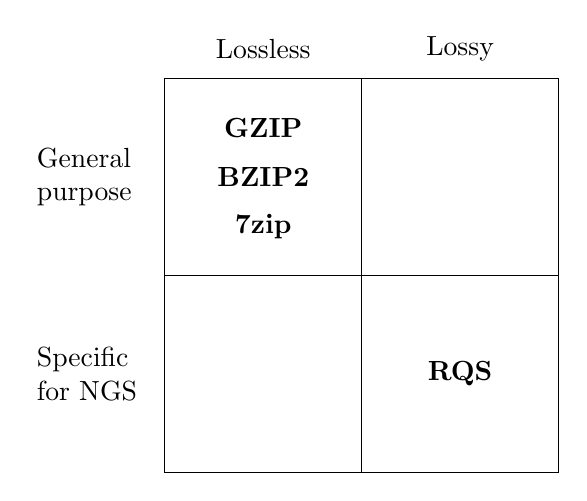
\begin{tikzpicture}
                \draw (0,0) -- (0,5) -- (5,5) -- (5,0) -- cycle;
                \draw (2.5,0) -- (2.5,5);
                \draw (0,2.5) -- (5,2.5);

                \node (lossless) at (1.25,5.375) [] {Lossless};
                \node (lossy) at (3.75,5.375) [] {Lossy};
                \node (specific) at (-0.625,3.75) [text width=2cm] {General \\ purpose};
                \node (general) at (-0.625,1.25) [text width=2cm] {Specific \\ for NGS};

                \node (gzip) at (1.25,4.375) [] {\textbf{GZIP}};
                \node (bzip2) at (1.25,3.75) [] {\textbf{BZIP2}};
                \node (7zip) at (1.25,3.125) [] {\textbf{7zip}};
                \node (rqs) at (3.75,1.25) [] {\textbf{RQS}};
            \end{tikzpicture}
        \end{figure}
    \end{frame}

    \begin{frame}{The FASTQ format}
    \end{frame}

    \begin{frame}{Phred quality score}
        \begin{definition}[Phred quality score]
            Let \(P_e\) be the estimated probability that a base call is
            incorrect. Then we define its \emph{Phred quality score} \(Q\) as
            \[
                Q = -10\log_{10}{P_e}\text{.}
            \]
        \end{definition}

        \vspace{0.5cm}

        This quantity is encoded in the Sanger FASTQ format as a single byte,
        where the character \texttt{\textquotesingle!\textquotesingle}
        represents the lowest quality while
        \texttt{\textquotesingle\textapprox\textquotesingle} is the highest.
    \end{frame}

    \begin{frame}{The RQS algorithm in brief}
        Yu, Yorukoglu and Berger \cite{YYB14} propose the following:

        \vspace{0.25cm}

        \begin{enumerate}
            \item Generate a dictionary \(\text{D}\) of all \(k\)-mers that appear
                with high multiplicity in a representative collection of reads.
            \item Let \(\gamma\) be a read. Its \(k\)-mers close to \(\text{D}\) in
                Hamming distance have nearly all of their quality score discarded.
            \item Compress the resulting high redundancy sequence with a general
                purpose lossless compression algorithm.
        \end{enumerate}
    \end{frame}

    \begin{frame}{The \textsc{Dict} algorithm}
        \begin{algorithm}[H]
            \caption{\textsc{Dict}}
            \begin{algorithmic}[1]
                \REQUIRE \(\text{C}, \text{k}, \text{r}\)
                \ENSURE \(\text{D}\)
                \STATE \(\text{D} \leftarrow \{\}\)
                \STATE \(\text{A} \leftarrow [0,\dots,0] \in \mathbb{N}^{4^\text{k}}\)
                \FOR{\(\text{x}\in \text{C}_\text{k}\)}
                    \STATE \(\text{A}[\text{x}]\pp\)
                \ENDFOR
                \FOR{\(\text{x}\in [4^\text{k}]\)}
                    \IF{\(\text{A}[\text{x}]\ge\text{r}\)}
                        \STATE \(\text{D}.\text{append}(\text{x})\)
                    \ENDIF
                \ENDFOR
                \RETURN \(\text{D}\)
            \end{algorithmic}
        \end{algorithm}
    \end{frame}

    \begin{frame}{The \textsc{MarkKmer} algorithm}
        \begin{algorithm}[H]
            \caption{\textsc{MarkKmer}}
            \begin{algorithmic}[1]
                \REQUIRE \(\text{x}, \text{D}\)
                \ENSURE \(\text{M}\)
                \IF{\(\Delta(\text{x}, \text{D}) > 1\)}
                    \STATE \(\text{M} \leftarrow [\text{false},\dots,\text{false}]\in\{\text{true},\text{false}\}^\text{k}\)
                \ELSE
                    \STATE \(\text{M} \leftarrow [\text{true},\dots,\text{true}]\in\{\text{true},\text{false}\}^\text{k}\)
                    \FOR{\(\text{y}\in\text{D}\mid\Delta(\text{x},\text{y}) = 1\)}
                        \FOR{\(\text{i}\in[\text{k}]\)}
                            \IF{\(\text{x}_\text{i}\neq\text{y}_\text{i}\)}
                                \STATE \(\text{M}_\text{i}\leftarrow\text{false}\)
                            \ENDIF
                        \ENDFOR
                    \ENDFOR
                \ENDIF
                \RETURN \(\text{M}\)
            \end{algorithmic}
        \end{algorithm}
    \end{frame}

    \begin{frame}{The \textsc{MarkRead} algorithm}
        \begin{algorithm}[H]
            \caption{\textsc{MarkRead}}
            \begin{algorithmic}[1]
                \REQUIRE \(\gamma, \text{D}\)
                \ENSURE \(\mathcal{M}\)
                \STATE \, \COMMENT Let \(\text{x}^\text{a}\) be the \(\text{k}\)-mer in \(\gamma\) starting at \(\text{a}\).
                \STATE \, \COMMENT Cover \(\gamma\) by \(\text{k}\)-mers \(\{\text{x}^{\text{a}_\text{1}},\dots,\text{x}^{\text{a}_\text{n}}\}\).
                \FOR{\(\text{i}\in[\text{n}]\)}
                    \STATE \(\text{M}^\text{i} \leftarrow \text{\textsc{MarkKmer}}(\text{x}^{\text{a}_\text{i}},\text{D})\)
                    \STATE \(\overline{\text{M}}^\text{i} \leftarrow [\text{false},\dots,\text{false}]\in \{\text{true},\text{false}\}^{\text{length}(\gamma)}\)
                    \FOR{\(\text{j}\in[\text{k}]\)}
                        \STATE \(\overline{\text{M}}^{\text{i}}_{\text{j}+\text{a}_\text{i}-1} \leftarrow \text{M}^\text{i}_\text{j}\)
                    \ENDFOR
                \ENDFOR
                \STATE \(\mathcal{M} \leftarrow \overline{\text{M}}^1 \lor \dots \lor \overline{\text{M}}^\text{n}\)
                \RETURN \(\mathcal{M}\)
            \end{algorithmic}
        \end{algorithm}
    \end{frame}

    \begin{frame}{The \textsc{SparsifyRQ} algorithm}
        \begin{algorithm}[H]
            \caption{\textsc{SparsifyRQ}}
            \begin{algorithmic}[1]
                \REQUIRE \(\gamma,\text{Q},\text{D},\text{Q}_{\text{threshold}}\)
                \ENSURE \(\text{Q}'\)
                \STATE \(\text{Q}' \leftarrow \text{Q}\)
                \STATE \(\mathcal{M} \leftarrow \text{\textsc{MarkRead}}(\gamma, \text{D})\)
                \FOR{\(\text{i}\in [\text{length}(\gamma)]\)}
                    \IF{\((\text{Q}_\text{i} > \text{Q}_{\text{threshold}}) \text{ \textbf{or} } (\mathcal{M}_\text{i} = \text{\text{true}})\)}
                        \STATE \(\text{Q}'_\text{i} \leftarrow \text{Q}_{\text{threshold}}\)
                    \ENDIF
                \ENDFOR
                \RETURN \(\text{Q}'\)
            \end{algorithmic}
        \end{algorithm}
    \end{frame}

    \begin{frame}{An example}
    \end{frame}

    \begin{frame}{Results}
        Results of compressing HG02215, chromosome 21 with \(\text{r} = 50\),
        \(\text{k} = 32\) and \(\text{Q}_\text{threshold} = 40\):

        \vspace{0.25cm}

        \begin{table}
            \centering
            \begin{tabularx}{\linewidth}{Xccc}
                \hline
                Method & Size & Bits/Q & F1 \\
                \hline
                Uncompressed & 273 MiB & 8.0000 & 1 \\
                GZIP & 143 MiB & 4.1923 & 1 \\
                BZIP2 & 133 MiB & 3.8791 & 1 \\
                \textbf{7zip (PPMd)} & \textbf{124 MiB} & \textbf{3.6269} & \textbf{1} \\
                \hline
                RQS + GZIP & 14 MiB & 0.3825 & 0.9914 \\
                \textbf{RQS + BZIP2} & \textbf{8.7 MiB} & \textbf{0.2540} & \textbf{0.9914} \\
                RQS + 7zip (PPMd) & 11 MiB & 0.2953 & 0.9914\\
                \hline
            \end{tabularx}
        \end{table}
    \end{frame}

    \begin{frame}{The implementation of \textsc{DICT}}
    \end{frame}

    \begin{frame}{An alternative implementation}
    \end{frame}

    \begin{frame}[allowframebreaks]{Bibliography}
        \bibliography{seminario.bib}
    \end{frame}
\end{document}
